\chapter{Methods and techniques}%
\label{ch:methods}

Since the works described in~\cref{ch:paper1,ch:paper2,ch:paper3} consist
of contributions related to the computational elucidation of reaction mechanisms,
this chapter presents an account of the relevant computational methods and
techniques used in the investigations,
with background and context given
for the various topics where appropriate.
A basic background on computational chemistry applied
to mechanistic elucidation is given in~\cref{sec:background-methods}.
Details about the methods used in the development of the \overreact software
package are given in~\cref{sec:overreact-methods}.

\section{Theoretical Background}%
\label{sec:background-methods}

Each of the steps in a proposed reaction mechanism is computational modelled
by optimizing the structures of reactants, transition states, intermediates, and products.
While the first two are minima on the potential energy surface, transition
states represent a local maximum on the potential energy surface connecting
reactants and products.
This characterizes transition states as saddle points and, therefore, requires
a different method of optimization than the other structures.
The potential energy surface can be regarded as a function from atomic coordinates to potential energy and,
as such, its existence is a result of the Born-Oppenheimer approximation,
where the electronic energy and wavefunction depends on the nucleus coordinates
only parametrically.
CITE BORN-OPPENHEIMER.\@
In this sense, nuclei are treated classically in this scheme, which is reasonable for most problems of interest in chemistry.
In contrast, other methods exist, where the nuclei are treated quantum mechanically as well,
but they are much more expensive.

In any case, optimization methods require an estimate of energies and gradients
of the potential energy surface.
There are many techniques available to accomplish that,
ranging from simple and low-cost semiempirical methods,
all the way throught highly accurate and expensive multideterminantal wavefunction calculations.
CITE, JACOB'S LADDER, HIERARCHY OF MODELS, ETC.\@
Most of these techniques require self-consistent field approximations, at least initially.

The works presented in this thesis made use of the most popular technique nowadays,
the density functional theory (DFT)
method~\cite{Hohenberg_1964,Kohn_1965,Perdew_2014,Kryachko_2014,Yu_2016} for
that.
A brief discussion of the theory can be found in~\cref{sec:dft}.

\subsection{Density functional theory (DFT)}\label{sec:dft}

This work has made extensive use of the density functional theory (DFT).
As such, a very brief introduction to the theory is provided here.
The interested reader is invited to read the cited references for more
details~\cite{Hohenberg_1964,Kohn_1965}.

The main equation used in the DFT is the following (\cref{eq:KS}):
%
\begin{equation}
	\left(-\frac{1}{2} \laplacian
	+ v_\text{ext}
	+ v_\text{eff}
	\right) \psi_i
	= \epsilon_i \psi_i
	\label{eq:KS}
\end{equation}
%
where $\psi_i$ is $i$th molecular orbital, $v_\text{ext}$ is the external
potential due to the atomic nuclei, $\epsilon_i$ is the electronic energy
of the $i$th orbital and $v_\text{eff}$ is the effective potential for a given
density functional (an approximation of the actual electron-electron
interaction).
This equation is analogous to the Hartree-Fock one~\cite{Szabo_1996}
and is solved self-consistently as well.
$v_\text{eff}$ consists of classical Coulomb interactions, as well as exchange
and correlation approximation
potentials~\cite{Perdew_2014,Kryachko_2014,Yu_2016}.
Other additive terms can appear in the potential as well, such as solvation
approximations when employed~\cite{Marenich_2009,Marenich_2012}.
The various ways of approximating the exchange and correlation potentials give
rise to a number of different density functionals developed in the
literature~\cite{Chai_2008a,Chai_2008b,Goerigk_2011,Arago_2011,Salzner_2011,Burns_2011,Minenkov_2012,DFT2016_poll}.

In the present work, all problems were treated by expanding the molecular
orbitals as a linear combination of basis functions centered at the atomic
nuclei~\cite{Szabo_1996,Helgaker_1997,Jensen_2012,Hill_2012}.
The literature on basis set functions is extensive~\cite{Ditchfield_1971,Hehre_1972,Hariharan_1973,Hariharan_1974,Gordon_1980,Francl_1982,Clark_1983,Frisch_1984,Binning_1990,Blaudeau_1997,Rassolov_1998,Rassolov_2001}.
We invite the interested reader to the references on each work for more about
the levels of theory used in each case.

IMPACTS OF DFT APPROXIMATIONS ON THE PES?\@

% TODO: check that citations follow the short compact convention e.g. [18-25]

\subsection{Single-molecule property predictions}\label{sec:optimizations}

\cref{eq:KS} allows us to obtain energy and gradient estimates (required for
the prediction of geometrical, thermochemical and kinetic properties) with a
reasonably good cost-effectiveness.
WHY, HOW, SUPPORT WITH WHAT?\@ CITATIONS!\@

The most basic property required for any computational study is the molecular
geometry.
It is obtained by minimizing the energy with respect to the atomic positions.
Commonly used and powerful family of optimization methods employed in the
literature is the \emph{quasi}-Newton method, where energies and gradients are
computed, while an approximation to the second-derivative matrix (also known as
a Hessian matrix) is updated at each step~\cite{Banerjee_1985,Schlegel_1987}.
CRUCIAL EQUATIONS SHOULD BE HIGHLIGHTED!\@

An approximation to the second-derivative matrix is employed in the algorithm
for efficiency, but the actual matrix can be computed after the minimization is
complete.
This matrix provides important information about the region in the potential
energy surface where the energy is minimum as we will see in the following.
EVERYTHING IS MISSING, EITHER REMOVE STUFF OR SHOW STUFF.\@
ALSO, CITATIONS ARE LACKING!\@
DON'T APPROACH THIS TANGENTIALLY.\@

\subsubsection{Transition state optimizations}\label{sec:ts-optimizations}
% TODO: the logical sequence is talk about ground-state optimizations first.
% Then move to transition state optimizations.

A structure to be a minimum on the potential energy surface means that any
displacement of the structure will result in an increase in the potential
energy.
As a consequence, its second-derivative matrix
is positive semi-definite (all eigenvalues are non-negative).
On the other hand, first-order saddle points are characterized by behaving as
a minimum with respect to all displacements of the structure except in a single
direction.
Displacement in this particular direction leads to a decrease in the potential
energy and is associated with a single negative eigenvalue of the
second-derivative matrix.
ADD A GRAPHICAL SCHEME TO SHOW THIS!\@
By calculating the second-derivative matrix, we can determine whether a structure
is a minimum, saddle point or otherwise.

Obtaining transition states can be done by a number of methods.
For instance, eigenvector following (\emph{EF})
method~\cite{Banerjee_1985,Schlegel_1987,Mauro_2005}
attempts to maximize the energy along a given promising direction, while
minimizing the energy along all other directions.
Another very much used is the \emph{STQN} method, developed
by~Peng~and~Schlegel~\cite{Peng_1993,Peng_1996},
It consists in obtaining an estimate of the transition state from the known
structures of reactants and products (QST2).
An associated method allows the use of a custom guess for the transition state
(QST3).
% TODO: one has to list the main characteristics of each method, advantages and disadvantages, etc.
% It is nice to have equations and/or schemes to highlight the most important things and is mandatory.
The method is useful since
i.\ knowledge of the transition state is optional,
ii.\ it avoids calculating the second-derivative matrix for each step.
The nudge-elastic band method is in the same vein as the \emph{STQN} method,
but attempts to minimize a discretized trajectory connecting reactants and
products along the transition state, and can thus make use of information about
this curve.

\subsection{Prediction of kinetics and thermodynamics for chemical reactions}

\subsubsection{Transition state theory}\label{sec:tst}

Transition state theory
is based on the idea that the reactant ground state complex is in equilibrium
with the transition state structure~\cite{TransitionStateTheory}.
It is summarized by the Eyring equation.

HAS TO BE REWRITTEN, BUT ONLY THE ESSENTIALS.\@

\subsection{When things go wrong:
	bulk effects}

Here are some situations where predictions become poor due to the fact that our
calculations are too small.

FLOATING PARAGRAPH!\@

\subsubsection{Determining \emph{pKa}s}\label{sec:pka}

WHY?\@
THIS MAKES THE TEXT NOT FOLLOW A CONCATENATED CHAIN OF THOUGHT.\@

In the computational prediction of \emph{pKa} values,
the direct dissociation approach (\cref{eq:pKa-equilibrium})
leads to problems in the evaluation of the solvated proton,
first because it is impossible to do electronic calculations for a zero-electron
system~\cite{Ding_2009,Sumon_2012}.
%
\begin{equation}
	\ce{HB (aq) <=>[$\emph{pKa} (\ce{HB})$] B^- (aq) + H^+ (aq)}\text{.}
	\label{eq:pKa-equilibrium}
\end{equation}
%
Second, due to the covalent nature of the interaction between the \ce{H^+} ion
and the surrounding environment, which leads to the formation of clusters such
as \ce{H3O+}, \ce{H5O2+}, etc.~\cite{Sumon_2012}.

One can employ the experimental proton solvation free energy
($-$1104,5~$\pm$~0,3~kJ/mol~\cite{Tissandier_1998,Marenich_2009}) in a
semi-empirical fashion, but the trustworthiness of the results is still highly
debated in the literature~\cite{Yang_2013}.
In fact, this often produces \emph{pKa} values that are far from the expected
for simple carboxylic acids, for instance.
Errors in the order of 7 \emph{pKa} units can be expected with this approach,
as can be found in the literature~\cite{Pliego_2002,Ding_2009}.
The major source of error can be attributed to the lack of explicit
solute-solvent interactions~\cite{Pliego_2002}.

A better approach is to use a relative determination method~\cite{Ding_2009}.
This avoids the problems associated with the direct dissociation approach
by calculating the associated problem of proton exchange with a known reference
acid, such as acetic acid~\cite{Goldberg_2002}:
%
\begin{equation}
	\ce{HA (aq) + B^- (aq) <=>[$\Delta{} G$] HB (aq) + A^- (aq)}\text{.}
	\label{eq:pKa-indireto}
\end{equation}
%
Since both sides of the~\cref{eq:pKa-indireto}
have the same net charge and, hopefully both acid and conjugated base are, in
general, of similar structure and size, favorable error cancelation is expected
in the Gibbs free energy ($\Delta G$).
The $\emph{pKa}(\ce{HA})$
can thus be written as a function of $\emph{pKa}(\ce{HB}, \text{exp.})$:
%
\begin{equation}
	\emph{pKa}(\ce{HA})~=~\emph{pKa}(\ce{HB}, \text{exp.}) + \frac{\Delta G}{\ln(10) R T}\text{.}
\end{equation}
%
It is customary that the error obtained by this method to be less than 1 \emph{pKa}
unit for many solutes and solvents~\cite{Ding_2009}.

\section{Chemical reaction mechanisms}

Hypothetical reaction mechanisms consist of
the interpretation of the available data for a chemical reaction
in terms of a model that is self-consistent.
Proposals for reaction mechanisms must be compared
with each other
and with the available experimental data.
Many different hypotheses for the same reaction can exist,
and,
after pruning the ones in disagreement with the available data,
it is still possible to have several different plausible models at hand.
Computational modelling of chemical reactions
provides one with a way of
formulating,
analyzing and
comparing hypotheses to each other,
to the literature and to the available experimental data.
This way,
one is able to come up with a ``most probable'' one.

\subsection{Bell-Evans-Polanyi principle}

The Bell-Evans-Polanyi (BEP) principle is a fundamental principle in the study
of chemical reactions.
It states that the more exothermic reactions usually have to overcome lower
reaction barriers and are therefore faster.

% TODO: equations,
% main features,
% scheme,
% missing!

It is customary to successfully extend this concept to exergonic reactions.
But since the largest contribution is the electronic energy,
it is reasonably
safe to apply the BEP principle (and Hammer's postulate,
as we will see later)
using electronic energies in the context of quantum chemistry calculations.

% TODO
IN THE NOTES.\@
CITATION.\@

\subsection{Hammond's postulate}

% TODO:
THIS IS CITED IN THE INTRO AS WELL

IN THE NOTES.\@
CITATION.\@

\section{Intramolecular and substitutional effects:
  a key step to understand enzyme-like catalysis}

Despite the great advancements in the developments of artificial enzymes~\cite{Breslow_1995},
the synthetic reproduction of the reaction rate accelerations attained by
natural enzymes is far from being reached.
To get there,
we will need a more detailed comprehension of the ways enzymes
work at the molecular level~\cite{Catalysis_in_Chemistry_and_Enzymology}.
Much effort has been put in this direction,
with at least six Nobel Prizes
awarded in this and related areas~\cite{Nobel_1929,Nobel_1946,Nobel_1957,Nobel_1975,Nobel_1997,Nobel_2013}.
These progresses show that the main source of acceleration in
enzymatic reactions is to be found in the events that accompany the
enzyme-substrate complex formation that leads to bond breaking and
formation~\cite{Catalysis_in_Chemistry_and_Enzymology}.
These events induce conformational changes in both substrate and enzyme,
which
enhances the interactions in the active site~\cite{Fischer_1890,Fischer_1894,Koshland_1958,Dafforn_1971,Kirby_1996}.
PICTURES OF REPRESENTATIVE SCHEMES!\@
As a result,
substrate active centers adequately orient themselves towards
their counterparts in the active site,
which leads to
i.\ a decrease in stability of the ground state (if compared with the
free substrate state),
ii.\ a lowering of the transition state energy (if compared with the
non-catalyzed reaction),
iii.\ energy relaxation through the formation of intermediates and
products.

These driving forces are also found in intramolecular reactions (\cref{fig:reacoes-intramoleculares}).
%
\begin{figure}[hbtp]
	\centering
	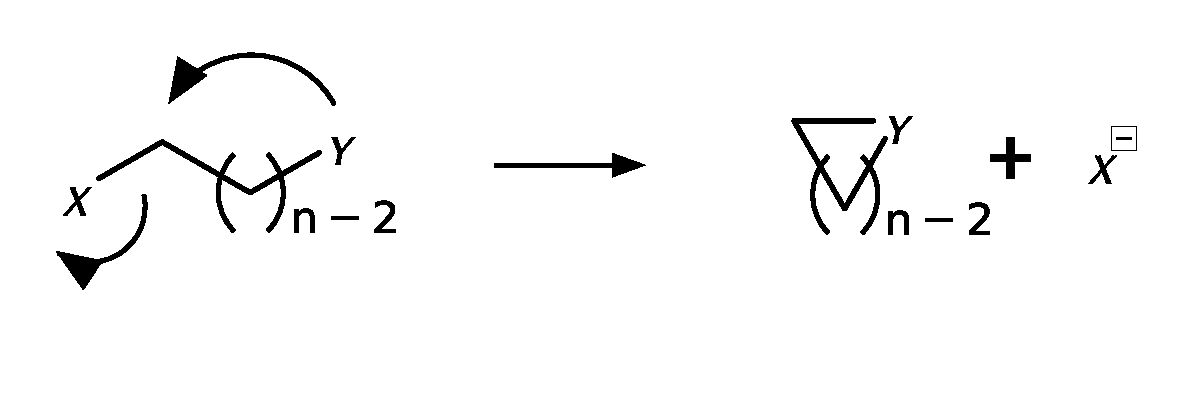
\includegraphics[width=.6\textwidth]{figures/reacao-intramolecular}
	\caption[Typical scheme of an intramolecular reactions]{
		Reaction scheme of a typical intramolecular reaction,
		whose products or
		intermediates are often cycles.
		Smaller rings ($n \le 4 $)
		tend to be disfavored by enthalpy,
		while larger rings ($n \ge 7 $)
		have less probable formation due to entropy.}%
	\label{fig:reacoes-intramoleculares}
\end{figure}
%
In fact,
the similarities between monomolecular enzymatic processes and
intramolecular reactions have been already recognized~\cite{Nilsson_1933,Bruice_1960b,Jung_1990}.
Despite the limitations of using intramolecular reactions as a model for
enzymatic reactions,
it is natural to suppose that the detailed understanding
of enzyme catalysis has,
as a prerequisite,
the ability to understand the
related processes in simpler systems.~\cite{Kirby_1972}.

We have studied some of these effects.
WHICH ONES?\@

% TODO: concatenate the results with those remarks.
% It's OK not to have it all!
% PAPER 1 => is peptide-like/enzyme-like? is intramolecular/substitutional?
% PAPER 2 => is peptide-like/enzyme-like? is intramolecular/substitutional?
% PAPER 3 => is peptide-like/enzyme-like? is intramolecular/substitutional?
% => \emph{\ce{N}}-alkyl substituted maleamic acids
Particular details concerning the intramolecular effects of geminal and
vicinal disubstitutions can be found in~\cref{ch:gem-vic-disubstitions}.

\section{Automatic determination of kinetics using \overreact}%
\label{sec:overreact-methods}

\overreact is an open-source library, software package and command-line
application for building and analyzing
homogeneous microkinetic models from first-principles
calculations~\cite{Schneider_2022,overreact2021zenodo}.
It propagates chemical reactions over time using only data available from
computational chemistry calculations.

All differential equations are and their parameters are inferred from a
reaction model and calculations provided by the user.
Simultaneous reactions are easily solved, including parallel and concurrent
reactions, pre-equilibration and even constant concentration reactants.

Furthermore, \overreact is able to take most of the relevant physics of the problem into
account in a semi-automated fashion.
This includes concentration effects, symmetries, quantum
tunneling, standard state corrections, implicit and explicit solvation, proper treatment
of energy contributions and dispersion corrections.
In most cases, in particular where solvation effects are weak, results matching
experimental data are obtained.

It is open source\footnote{Code is available at
	\url{https://github.com/geem-lab/overreact-guide}.}, free of charge, available through the Python Package Index (PyPI) and is
distributed under the MIT license.
An online user manual is also
available\footnote{The user guide can be found at \url{https://geem-lab.github.io/overreact-guide/}.}.

USE THE SI FROM THE PAPER TO ADD CONTENT HERE.\@

\section{Thermochemical partition functions}

It is possible to make use of computational calculations to obtain
thermochemical data and, in particular, the thermochemical partition
functions.
This is routinely achieved by standard computational chemistry packages.
This data can be used to estimate the thermodynamic properties of molecules and
whole systems.

Não apenas seus autovalores nos permitem checar se uma otimização alcançou de fato um mínimo local, mas importantes funções de estado termodinâmicas são acessíveis através da matriz hessiana, valendo-se da aproximação QRRHO para gases ideais.

teoria do estado de transição~\cite{TransitionStateTheory}. %(\cref{sec:tst}).

\section{Why predicting chemical reactions is hard}

Perfect prediction of chemical reactions is an unforgiving problem.
Since reaction rate constants depend exponentially on the activation Gibbs' free energy,
small deviations on the latter exponentally increase errors on the latter.
As such, given an activation energy estimate $\Delta G^\ddagger$
on the true value $\Delta \widehat{G}^\ddagger$
with error $\epsilon$,
%
\begin{equation}
	k = \kappa \frac{k_B T}{h} e^\frac{- \Delta G^\ddagger}{R T}
	= \kappa \frac{k_B T}{h} e^\frac{- \left(\Delta \widehat{G}^\ddagger + \epsilon\right)}{R T}
	% = \kappa \frac{k_B T}{h} e^\frac{- \Delta \widehat{G}^\ddagger}{R T}
	% e^\frac{- \epsilon}{R T}
	= \widehat{k} e^\frac{- \epsilon}{R T}
\end{equation}
%
where $k$ and $\widehat{k}$ are the predicted and true chemical reaction constants, respectively.
Thus, at room temperature, an error of 1.36--2.73~\kcalmol gives rise to 10--100$\times$ error
in the reaction rate constant, with larger errors found in lower temperatures.
This is particularly important, as popular DFT methods commonly achieve accuracies of
2--3~\kcalmol for many molecules~\cite{Becke_2014,Bogojeski_2020}.
Moreover, an error of 0.41~\kcalmol produces a twofold error in the constant.
This goes to show that the so called ``quantum chemical accuracy'' of
$<$1~\kcalmol~\cite{Bogojeski_2020}
is not enough for the prediction of chemical reactions on par with experimental results.
It goes without saying that this gives rise not only to a demand
for more precise quantum chemical methods,
but also for methods aiming at mitigating the effect of such errors
in computational predictions of chemical reactions.

One might go one step further and investigate how this error in the reaction rate constant
is related to individual errors in activation enthalpy and entropy errors.
%
\begin{equation}
	k = \kappa \frac{k_B T}{h} e^\frac{- \Delta H^\ddagger}{R T}
	e^\frac{  \Delta S^\ddagger}{R}
	= \kappa \frac{k_B T}{h} e^\frac{- \left(\Delta \widehat{H}^\ddagger + \chi\right)}{R T}
	e^\frac{        \left(\Delta \widehat{S}^\ddagger + \sigma\right)}{R}
	% = \kappa \frac{k_B T}{h} e^\frac{- \Delta \widehat{H}^\ddagger}{R T}
	% e^\frac{  \Delta \widehat{S}^\ddagger}{R}
	% e^\frac{- \chi}{R T}
	% e^\frac{  \sigma}{R}
	= \widehat{k}
	e^\frac{- \chi}{R T}
	e^\frac{  \sigma}{R}
\end{equation}
%
The above suggests that, all things equal,
errors in the predicted activation entropy dominate at high temperatures,
while being less significant
than activation enthalpy errors at low temperatures.
The balance between the two will on the other hand depend on the actual reaction at hand.

\section{``First-principle'' calculations}

Strictly speaking, computational first-principle calculations encompass
methodologies that do not use experimental data either in their development or
application.
Broadly speaking, the first-principle calculations can be referred to
wavefunction or density-functional theory (DFT) calculations.

Os perfis reacionais resultantes são suficientes para a predição de parâmetros
cinéticos e termodinâmicos das reações, que foram comparados aos resultados
disponíveis na literatura. %(\cref{sec:tst}).

\subsection{Quantum tunneling effects}

Hydrogen abstraction reactions (HAA) comprise a class of reactions where
quantum tunneling is often very important~\cite{Bim2018}.
A particular group therein is the homolysis of \ce{C-H} bonds by strong
oxidants, which oftentimes the rate-limiting step in many transformations, and
a particularly key step in the substrate activation by numerous
metalloenzymes~\cite{Bim2018}.

\section{Microkinetic modelling}

Microkinetic modelling is a technique used to predict the outcome of complex
chemical reactions.
It can be used to investigate the catalytic transformations of molecules by
propagating a system of ordinary differential equations modelling the chemical
reactions.

The technique can be made first-principle by making use of pure computational
chemistry predictions.
It is able to take into account effects that sole use of Gibbs' free energies
are not able to, such as concentrations of species and complex time dynamics.

\subsection{Design}

\overreact is a second iteration on an earlier attempt to build a
homogeneous microkinetic analyzer from first-principles
calculations~\cite{pyrrole2019zenodo}.
Some things were learned from that first attempt:
i.\ data is relatively easy to obtain from computational chemistry calculations,
but it is not always in its optimal form;
ii.\ solving differential equations is relatively easy in general, but hard to
make it work for a wide range of problems mostly due to stiffness of the
equations;
iii.\ transforming knowledge about chemical structures into knowledge about the
chemical reactions is hard to be done in an automated fashion;
iv.\ having a good pipeline for data processing makes it easy to add new
features to the system.

\subsection{Automatic differentiation}

Instead of employing numerical differentiation, whose precision depends on the
particular step size, automatic differentiation can be used to produce
analytical derivatives in a precise, efficient and automated way.

One conceptually simple way of doing this is by \emph{forward differentiation}
through dual numbers, where the real values are extended by an infinitesimal
part in a trick that is not far from the concept of imaginary numbers.
The pair of numbers can be added component-wise, and form a commutative algebra
by making use of a simple multiplication rule that follows from the property
$\epsilon^2 = 0$:
\begin{equation}
	(a, b) * (c, d)
	\equiv (a + b\epsilon)(c + d\epsilon)
	= a c + (a d + b c)\epsilon
	\equiv (a c, a d + b c)
\end{equation}
It is not hard to show that, by extending the domain of any real polynomial to
dual numbers, one obtains
\begin{equation}
	P((a, b)) \equiv P(a + b\epsilon) = P(a) + b P'(a) \epsilon
\end{equation}
where $P'(a)$ is the \emph{analytic} derivative of $P(a)$.

\overreact employs a sligthly more complex scheme called
\emph{backward differentiation}, available through Google's JAX library, that
is more efficient for functions of many variables.

% TODO: highlights
Used energy correction of 3.2~kcal~mol$^{-1}$ for RMSE of 4.97~mM;\@
additional approximations (Eckart,
\emph{quasi}-rigid rotor-harmonic oscillator) applied.

% TODO: transform in a methodology highlight only
We showed how
acetic acid-acetate concentrations could be estimated using a combination of \emph{ab initio} calculations and experimental pK$_a$ values.
Algorithm creates fictitious reaction rate constants that guarantee equilibrium is satisfied,
allowing simultaneous study of both fast reactions and equilibria.
Equilibria can provide qualitative insight and be used to obtain Boltzmann populations with constraint optimization.
We estimated acetic acid-acetate concentrations using a combination of \emph{ab initio} calculations,
experimental pK$_a$ values and \ce{H+} concentration constraining.
Optimizations and frequencies for \ce{AcOH(aq)} system performed concluding with predictions of reaction concentrations of both solvation energies.
\overreact{} produces the expected result if given precise energy values.
% TODO: transform in a methodology highlight only

% TODO: things from the quali
% Mecanismos foram validados com base na concordância relativa aos respectivos resultados experimentais~\cite{Kirby_1972,Jung_2005}.
% A termoquímica relevante foi calculada à condição de temperatura e pressão ambientes (298.15~K e 1~atm).
% Determinações de \emph{pKa} dos compostos estudados também foram realizadas com
% relação ao ácido acético,
% de acordo com o esquema de
% \citeauthor{Ding_2009}~\cite{Ding_2009} (\cref{sec:pka}).

% Cálculos foram realizados com o programa Gaussian~09C.01~\cite{g09} e com o funcional da densidade
% % PBE0~\cite{Perdew_1996,Perdew_1997,Ernzerhof_1999,Adamo_1999}
% \emph{wB97XD}~\cite{Chai_2008a,Chai_2008b} (\cref{sec:funcionais}),
% que foi
% utilizado em conjunto com funções de base de Pople de qualidade triplo-$\zeta$
% com funções difusas e polarizações em todos os átomos
% (\emph{6--311++G**}~\cite{Ditchfield_1971,Hehre_1972,Hariharan_1973,Hariharan_1974,Gordon_1980,Francl_1982,Clark_1983,Frisch_1984,Binning_1990,Blaudeau_1997,Rassolov_1998,Rassolov_2001},~\cref{sec:basis-functions}).
% Todos os cálculos levaram em consideração efeitos de solvatação aquosa através
% do uso do \emph{SMD},
% desenvolvido por \citeauthor{Marenich_2009} (\cref{sec:implicit-solvation}).
% De forma a se investigar o efeito da geometria do estado fundamental,
% uma
% análise conformacional dos compostos foi empregada,
% usando o programa Open
% Babel 2.4.1~\cite{O_Boyle_2011} com o \emph{PM7} (MOPAC2016~\cite{MOPAC},~\cref{sec:conformational-analysis}).

% Estruturas eletrônicas dos compostos serão estudadas à luz dos \emph{NBO}
% (\cref{sec:nbos}).

% em particular para se correlacionar o efeito cinético da substituição
% \begin{enumerate*}[label=(\roman*)]
%   \item com eventuais flutuações de hibridização dos carbonos da ponte~\cite{Bent_1961} e
%   \item com a magnitude da repulsão estérica entre substituintes e grupos reativos.
% \end{enumerate*}

% Para tanto será utilizado o programa NBO~5.9~\cite{NBO5.9} acoplado com o programa Gaussian~09C.01~\cite{g09}.
